\section{Ejercicio 1}

Para la resolución de este ejercicio, se requería programar un tipo de tarea \emph{TaskConsola} donde debía realizar $n$ llamadas bloqueantes, cada una con una duración aleatoria de valor $random\_num: bmin \leq random\_ num \leq bmax$.
~
Para lograr esto, ciclamos \emph{n} veces en el cual, en cada iteración generamos un número pseudoaleatorio utilizando la función \textbf{rand()} de la forma:

\begin{center}
	\textbf{random\_num = bmin + rand() \% (bmax - bmin + 1)}
\end{center}

Una vez hecho esto, realizamos la llamada bloqueante con la cantidad de ciclos definida por ese valor pseudoaleatorio creado y luego ejecutamos un tick.

\begin{figure}[!h]
	\begin{center}
		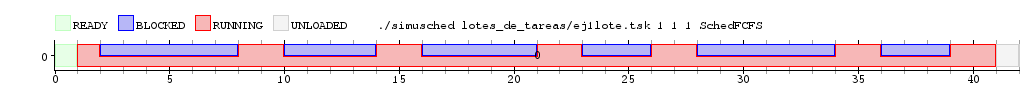
\includegraphics[width=500px]{imagenes/ej1.png}
		\caption{\emph{TaskConsola} corriendo con $n = 6$, $bmin = 3$ y $bmax = 7$.}
	\end{center}
\end{figure}
